Gang er en fysisk bevægelse, som benytter involverer hele kroppen til at koordinere bevægelsen. Den følgende beskrivelse af én gangcyklus, tager udgangspunkt i beskrivelsen af bevægelserne for det højre ben. Bevægelserne er dog tilsvarende for det venstre ben. \citep{VaughanDavisOConnor1992}

En gangcyklus begynder når en fod har opnået kontakt med underlaget. Når denne cyklus er påbegyndt, inddeles cyklussen endvidere i to faser; standfasen og svingfasen, hvilket fremgår af nedenstående figur. 

\begin{figure}[H]
	\centering
	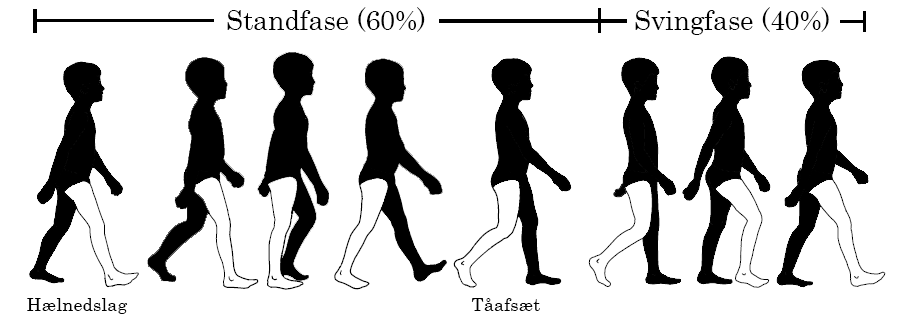
\includegraphics[scale=0.55]{figures/bProblemloesning/gang_cyklus.png}
	\caption{Figurtekst… \fxnote{SKAL MODIFICERES} \cite{ VaughanDavisOConnor1992}}
	\label{fig:gang_cyklus}
\end{figure}

Som det fremgår af \figref{fig:gang_cyklus}, er standfasen svarende til cirka 60\% af en gangcyklus. Dette skyldtes, at standfasen involverer 
